The primary objectives of the motion model are global synchronization, Web
availability and simplicity for Web developers. Global synchronization implies
media synchronization across Internet. Web availability essentially means
that no additional assumptions can be introduced for media synchronization. If a Web browser is able
to load an online Web page, it should also be able to synchronize correctly.
The model proposed for this can be outlined in three simple steps:

\begin{itemize}
\item{Media clock and media controls are encapsulated in one concept, and
represented as a stateful resource. This chapter uses the term \emph{motion}\footnote{\emph{motion} as in \emph{motion pictures}. \emph{Moving through media} still remains a good way to conceptualize media experiences, not least as media experiences become virtual and immersive.
} for this
concept.} 
\item{A \emph{motion} is an online resource, implying that it is hosted by a
server and identifiable by URLs.}
\item{\emph{Media components}\footnote{\emph{media component:} anything from a simple $<div>$ tag with text, to a highly sophisticated media player or multimedia framework.
} synchronize themselves relative to online motions.}
\end{itemize}

That is all. The main idea is that media synchronization should be a
consequence of connecting multiple media components to the same online motion.
This way, rich synchronized multi-device, multimedia may be crafted simply by
connecting relevant media components to the same online motion.

\begin{figure}[h]
%\sidecaption
\centering
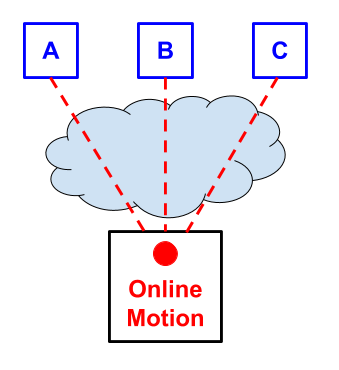
\includegraphics[scale=.4]{fig/motion-model.png}
\caption{Media components on three different devices (A,B,C), all connected to an online motion
(red circle). Media control requests (e.g. pause/resume) target the online motion and are transmitted across Internet (light blue cloud). The corresponding state change is
communicated back to all connected media components. Each media component
adjusts its behaviour independently.}
\label{fig:model}
\end{figure}

Importantly, the practicality of the motion model depends on Web developers
being shielded from the complexities of distributed synchronization. This is
achieved by having a \emph{motion} object\footnote{ A $<motion/>$ tag is not
appropriate, as motions do not require predefined visual representation.
Instead, media components, especially those concerned with media control, may
provide visual representations for motion, e.g. progress bar for media offset,
or buttons for play and pause. } locally in the Web browser. The motion object
acts as an intermediary between media components and online motions, as
illustrated by Fig.~\ref{fig:model-2}. This way, the challenge of media synchronization
is divided in two parts.

\begin{itemize}
\item{\emph{motion synchronization}: motion object precisely synchronized with online motion (Internet problem).}
\item{\emph{component synchronization}: media component precisely synchronized with motion objects (local problem).} 
\end{itemize}


\begin{figure}[h]
%\sidecaption
\centering
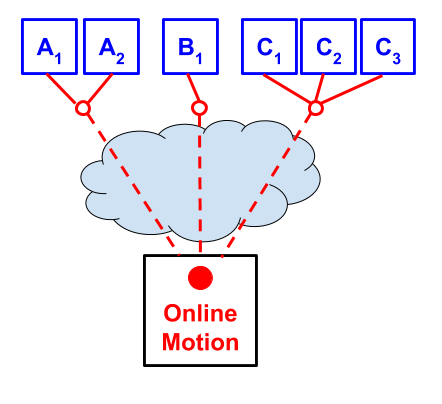
\includegraphics[scale=.4]{fig/motion-model-2.png}
\caption{Motion objects (red unfilled circles) mediate access to online motion. Motions objects may be shared by independent mediacomponents within the same browser context.}
\label{fig:model-2}
\end{figure}

\emph{Motion synchronization} ensures that motion objects connected to the same
online motion are kept precisely synchronized. The logic required for motion
synchronization could be supported by Web browsers natively (if standardized),
or imported into Web pages as an third party JavaScript library.
Implementations of motion synchronization would also include useful
optimizations, such as sharing the same motion object between multiple media
components [FIG], as well as multiplexing communication for different
online motions over a single connection. Motion synchronization is outlined in
Sect.~\ref{sec:motionsync}.

\emph{Component synchronization} implies that a media component continuously strives
to synchronize its activity relative to a motion object. As such, component
synchronization is a local problem. Media components always interface with
motion objects through a well defined \emph{Motion API} (see Sect.~\ref{sec:motionapi}).
Sect.~\ref{sec:compsync} discusses component synchronization in
further detail.
